\chapter{SegMatchAE}
\label{chap:ae}

This Chapter details the work following the implementation of SegMatch. In this part of the project, the goal was to design and implement a learning descriptor, that would improve the quality of descriptions and matches.\\

\section{Extending Segment Matching}
\label{sec:ae-intro}
%TODO

Recent work is showing neural networks as a versatile and promising machine learning technique. Despite initial promise in the years following the invention of the Perceptron \cite{perceptron} in 1958, neural networks did not show useful results, or superiority to other machine learning algorithms on many problems for some time. In the recent years (2006-) however, breakthrough results in the fields of audio \cite{wavenet}, visual \cite{inception}, natural language processing \cite{nlp}, game-agent \cite{alphago}, to cite a few, have led to increased research effort and adoption in consumer and business technologies.\\

There is little doubt that neural networks can also be useful in the robotics field. With this in mind, and based on pre-existing research on classifying 3D segments using neural networks (see Subsection~\ref{subsec:voxnet}), it was decided that neural networks were an ideal candidate for improving SegMatch performance.\\

As seen in Chapter \ref{chap:segmatch}, description shows a significant potential for improvement. Hand-crafted features are often heuristic based, and tedious to design and experiment on. In addition, the description task shares similarities with 3D object classification, which is a current subject of machine learning research. Thus, the description module was selected as the section of the algorithm to be supplemented with a neural network model.\\

\section{Neural Networks for 3D Segment Recognition}
\label{sec:neural-nets}

\subsection{Artificial Neural Networks - A Primer}
\label{subsec:primer}

In this subsection, the reader unacquainted with neural networks can find a short summary of many concepts used in this project.  
Another goal of this subsection is to define some terms used later in this chapter, such as \textit{hidden layer}, \textit{backpropagation}, etc, which are relevant for understanding the proposed work.

\subsubsection{Artificial Neural Network}
\label{subsubsec:simple-model}

The simplest artificial neural network model is a series of layers, each containing a few artificial neurons. Inputs get propagated forwards through the network. Inspired by the way signals flow through a neuron's many synapses, each input to a neuron is multiplied by a particular weight. All of a neuron's weighted inputs are added together, a bias term is added, and the result is passed through the neuron's activation function $f(x)$, which can be for example the sigmoid function. The resulting value is the neuron's output.\\

In the \textit{fully-connected} layer architecture, all neuron outputs of a layer become the inputs to all neurons in the next layer. The input values to the algorithm are treated as though they were neuron outputs of an 'input' layer, and fed directly into the inputs of the first neuron layer.\\

The last neuron layer is called the 'output' layer, and its neurons activations form the output values of the algorithm. All layers between the 'input' and 'output' layer are referred to as 'hidden' layers.\\

In the simplest case, learning is achieved through \textit{backpropagation} of the output error. That is, a training example is given as input to the network, and successive layer activations are calculated, until the model output. The error between the model output and the target output (the ideal output of the network, which must be known in advance for all training examples) is calculated. The gradient of this error w.r.t. the model parameters (weights and biases) is then computed, propagating backward from the output neurons all the way back to the first input layers. All parameters are then updated by a small amount according to the opposite direction of this gradient (this simple update rule is referred to as \textit{Gradient Descent}). When this process is repeated several times and for many examples, the model improves its prediction capabilities for the training data. If this training data is sufficiently general, this process often leads to model to learn generally useful relationships within the data, which allow it to also improve its prediction capabilities on data it has never been presented with.\\

\subsubsection{Deep Networks}

An arbitrary amount of hidden layers can theoretically be stacked behind each other. Networks consisting of many hidden layers are referred to as 'deep' neural networks, and are in practice often able to capture complex relationships more efficiently within their logical pathways than 'shallow' networks.\\

As is often repeated in the context of artificial neural networks, a shallow network consisting of a single neural network, given that it has infinitely many neurons, can theoretically compute any function $f(inputs) = outputs$. In practice however, deeper networks are often used when attempting to compute complex functions.\\

In addition to simply having more layers, deep neural networks often have architectures and particularities which differ from the simple model presented in the previous Subsubsection. This is due in part to instabilities which arise when backpropagating the error through many layers.\\ 

\subsubsection{Convolutional Neural Networks}

The intuition behind convolutional neural networks is to take advantage of repeating patterns in the model input. A neural network model which takes a whole image's pixel values as inputs, for example, is likely to be presented with underlying relationships in the input data which are repeated in several locations of the input.\\

Convolutional layers create small neural network layers, with a reduced amount of inputs $n\times n$ (for example, $n = 5$), commonly referred to as filters. A single filter is applied at each position in the full layer-input $N\times N$, taking the $n\times n$ surrounding values as filter inputs, and outputting a single value.\\

Filters can also be applied with \textit{strides}, meaning that the filter skips over every k input positions, leading to a reduced size layer-output.\\

Thus convolutional layers allow useful pattern learning in the input, with few parameters. On the other hand, convolutions generally require heavier computation. They have shown good results in many tasks, and are quite widespread especially with tasks where repeated patterns are expected in the input (computer vision, audio).\\

\subsubsection{Pooling}

\textit{Pooling} layers reduce the size of their output by applying a pre-determined filter (i.e., which has no learnable parameters) at every position with a stride. For example, a 2x2 \textit{Max pooling} layer has a single max filter of size 2x2, which simply returns the max value of its inputs. This filter is applied with a stride of 2, resulting in a downsampled output.\\

\subsubsection{Other Architectures}

It should be mentioned that there are yet many other architectures of neural networks showing good results in current research, to name a few: Recurrent Neural Networks (RNN), Dynamic Neural Computers (DNC), Residual Networks (ResNets) and many more. These will not be discussed in this thesis.\\

\subsubsection{Gradient Descent Optimization}

Gradient Descent (mentioned in the ``Artificial Neural Network'' Subsubsection) is a simple algorithm, but not the most efficient, for finding local minima for the error function in the many-dimensional model parameter space.\\

Optimizers are modified Gradient Descent algorithms which help navigate the many-dimensional parameter space more efficiently when performing the backpropagation step. They do so by implementing methods such as artificial momentum, looking ahead of the current position in this parameter space, and other techniques. This allows the backpropagation algorithm to reach local minima of the error function with fewer learning steps.\\

In this project, the neural networks were trained by using the Adaptive Moment Estimation (ADAM) optimizer. The ADAM optimizer computes learning rates for each parameter in the model, and adapts those rates based on previous fluctuations of gradients and previous parameter update values.  
More information is available in \citet{adam}, where empirical results of ADAM's learning speed-up are also shown.

\subsection{Neural Network Input}
\label{subsec:NNinput}

Feedforward neural networks take a fixed number of inputs. However, 3D segment data is usually in the form of a list of 3D points, each with 3 coordinates $(x,y,z)$. The amount of points varies from segment to segment.\\

A common way to adapt the data to the input size is padding, where the input size of the model is set to the largest possible size in the data, and a fixed value is attributed to 'missing' inputs, signaling the network that these inputs are to be ignored.\\

In the case of 3D segments, a list of points is intuitively not the best representation of the underlying 3D data, as it has an intrinsic order which in practice is arbitrary (i.e., there is no reason for the first point to be first). Networks however tend to try to learn relationships between inputs depending on their positions, where in this case (the input being an unordered list of points) there is none.\\

Voxelizing the 3D segments can yield occupancy grids of fixed size. In addition, the order of the values inside a voxel representation matters (the first point has coordinates (0,0,0), the second (0,0,1), etc.). These properties are ideal for convolutional networks. The downside is that precise geometrical information is lost with low voxel grid resolutions.\\

The proposed process of voxelizing a 3D segment is as follows:

\begin{algorithm}
  \caption{Voxelizing a 3D segment}
  \begin{algorithmic}[1]
    \State Initialize $O$, an NxNxN occupancy grid, with every voxel value set to 0.
    \State Decide on a transformation $T$ mapping $(x,y,z) \to (l,m,n)$, $x,y,z$ being coordinates in the 3D segment frame, and $l,m,n$ indices of the occupancy grid. In our case, T maps the segment bounding box to the occupancy grid. Each dimension $x,y,z$ of the bounding box is divided into n equal intervals.
    \For {each point $p_i$ in the segment of size $n$, $i \in [1,n]$}
    \State Find the position $(l,m,n)$ in $O$ in which $p_i$ falls according to $T$.
    \If {$O_{l,m,n} = 0$} \State set $O_{l,m,n} = 1$
    \EndIf
    \EndFor
  \end{algorithmic}
\end{algorithm}

\subsection{Neural Networks for 3D Segment Classification}
\label{subsec:voxnet}

Maturana and Scherer \cite{voxnet} use 3D convolutions in their VoxNet model, in order to classify 3D segments. The motivation behind VoxNet is to determine if advances made through convnets in computer vision tasks could extend to 3D data.\\

VoxNet takes a 32x32x32 occupancy grid as input, and outputs a softmax classification of the segment.  
Its first two layers are convolutions, with respectively 32 5x5x5 filters and 32 3x3x3 filters, a 2x2 max pooling layer, a fully connected layer of size 128, and a softmax fully connected output layer of size $K$, $K$ being the number of possible classes to draw a prediction from.\\

Maturana and Scherer found that VoxNet performs at state-of-the-art accuracy.


\subsection{Unsupervised Learning with Neural Networks}
\label{subsec:autoencoder}
%TODO

In the SegMatch case, the present task does not require classification but description. As discussed in Section ~\ref{sec:description}, the description scenario entails no known targets such as in classification, but rather heuristics for relative positions of the segment descriptions. That is to say, the correct output of our model for a given segment is not known in advance. In addition, even if the true ideal description of each segment could be known in advance, there is as of yet no 3D segments dataset with those target descriptions available, which is necessary for supervised training. Creating such a dataset would be a time-consuming task and was not the goal of this project. On top of this, such a dataset might become obsolete as sensor-technology evolves, or when using a different segmentation algorithm.\\

For these reasons, unsupervised training was deemed a more promising method. In unsupervised training, no ground-truth is required to train the model, it can be trained with each new example extracted from the environment, with no processing before-hand.\\

An example of an unsupervised neural network architecture is the Autoencoder, in which an encoder network compresses the input to a small-dimensional representation, and a similar-sized decoder network attempts to decompress the representation back into the original input. The intuition is that, should the network be able to do this for many examples it has not seen before, it will have successfully learnt a meaningful representation of the inputs in n-dimensional space. As the output target is identical to the input, no ground-truth information is required for the training examples, which means that no hand-labeling or label databases are necessary.\\

Whereas other types of unsupervised models exist, such as Adversarial Networks, they do not fall within the scope of this thesis report.

\subsection{Variational Bayes Autoencoder}
\label{subsec:variational-bayes}
%TODO

Kingma and Welling \cite{variational-autoencoder} present a modified autoencoder architecture. The variational Bayes autoencoder does not only predict an n-value representation at the encoder output (the n-dimensional space at the encoder output is also referred to as the \textit{latent space}), but parameters to a probabilistic distribution of each of those values. In simplified terms, it can be designed to predict means and variances in the case of a standard distribution. A value is then randomly sampled from each distribution, and the resulting n-values are passed to the decoder network.\\

The second contribution in \citet{variational-autoencoder} is to introduce a cost function for the autoencoder output which not only penalizes errors in the reconstruction (through for example cross-entropy loss between output prediction and true probability), but also the Kullback–Leibler divergence of the latent space prediction w.r.t. the true prior distribution in latent space. \citet{variational-autoencoder} show that these modifications to the standard autoencoder result in superior prediction performance and learning efficiency.

\section{3D Autoencoders for Segment Matching}
\label{sec:ae-implementation}

During the course of this project, we designed and implemented an autoencoder model in Tensorflow \cite{tensorflow}, and included it in the SegMatch algorithm.\\

The model comes in two architectures, which we refer to as \textit{fast} and \textit{accurate}, respectively without and with 3-dimensional convolutions.\\

As depicted in Fig.~\ref{fig:architecture}, the fast architecture consists of the input layer, two fully connected layers (400 hidden neurons each), and a fully connected output layer of size $k$, $k$ being the dimensionality of the latent space.

\begin{figure}
  \centering
  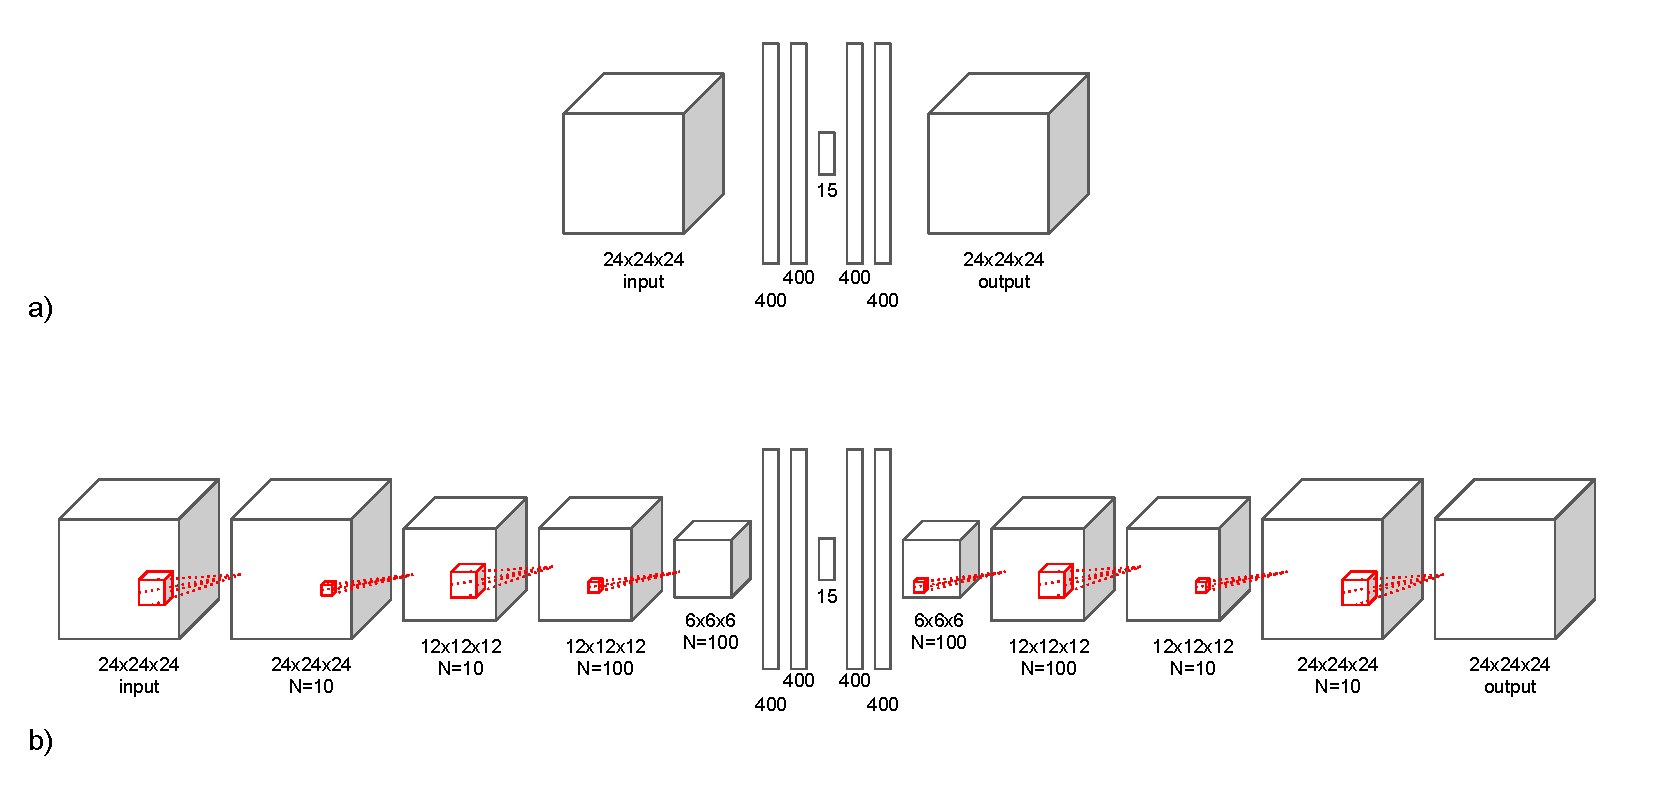
\includegraphics[width=5.2in]{images/architecture.pdf}
  \caption{The SegMatchAE autoencoder architectures. a) The fast architecture, with both the encoder and decoder sections of the model being composed of two fully connected layers. b) The accurate architecture, with two added 3D convolutional layers for both encoding and decoding, with a max-pooling step after each convolutional layer.}
  \label{fig:architecture}
\end{figure}

In both architectures, the latent space size is set to 15. The value of 15 was selected experimentally, see Appendix, Section \ref{sec:latent_space_size}. To these 15 values predicted by the autoencoder for segment representations, are concatenated 3 dimensional scales, for $x$, $y$, and $z$, which are calculated during voxelization. These are added because the voxelization step scales all segments to fit inside the occupancy grid. Thus, the autoencoder is given dimensionless input in $x$, $y$, and $z$ directions. As such, unless the autoencoder guesses the common size of segments based on other indicators (there is reason to believe that it does not: such information would not improve its reconstruction accuracy, nor do we give it any data during training that would allow such properties to be learnt), size information of the segment would be lost. This gives the SegMatch autoencoder descriptor a total of 18 features.\\


\subsection{Training}
\label{subsec:ae-training}

A model was trained for each architecture, fast and accurate.  
The training data were segments extracted during SegMatch runs on the KITTI datasets (drive 18, 20, 27), which results in over 6000 unique 3D segments.\\

In addition, each segment was rotated along the vertical axis according to 36 rotation angles distributed linearly from 0 to 2$\pi$, resulting in a total of over 216000 examples. The first 400 original segments and their rotations - a total of 14400 examples - were used as a validation dataset, and the remaining were used as training examples.\\

With GPU enabled (GeForce GTX 980 Ti), a single training epoch on this dataset takes on average 500 seconds for the fast model, and 1000 seconds for the accurate model.\\

\section{Performance}
\label{sec:ae-performance}

On a desktop computer with no GPU, the fast model requires on average 100 ms to encode 100 segments.
The accurate model requires on average 20 seconds to encode 100 segments. With GPU enabled (GeForce GTX 980 Ti), a 20x speedup is measured on average for the accurate model during training. For encoding, a more modest speedup of around 5x is observed.\\

Voxelizing 100 segments requires on average 20 ms.\\

In addition, the total autoencoder descriptor latency is affected by some data transfer overhead between python and C++. We were able to reduce the transfer overhead (C++ to python, then python to C++) to an average of 250ms for 100 segments.\\

As such the total time required for description when using the fast model within SegMatchAE was measured as 350ms on average, well within the required latency times required to run SegMatch online on all our available datasets.\\

\section{Results}
\label{sec:ae-results}

\subsection{Segment Reconstructions}

As explained in Subsection \ref{subsec:autoencoder}, the autoencoder model encode its 3d segment input into a description vector, and then decodes this description back to a 3d segment. This process is referred to as reconstruction. Our measurements show greater reconstruction accuracy for the accurate model architecture, as expected (see Fig.~\ref{fig:trainingcost}, \ref{fig:conv-reconstr}, and \ref{fig:noconv-reconstr}).\\

\begin{figure}
  \centering
  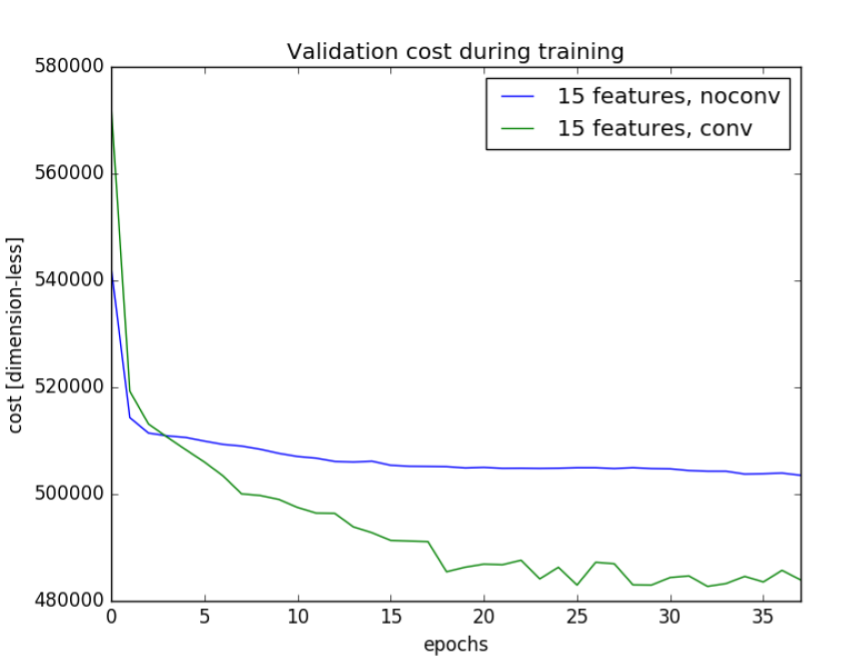
\includegraphics[width=3.2in]{images/trainingcost.png}
  \caption{Comparison of validation cost for the fast and accurate architectures, when the same training regime is applied to both, shows that the accurate architecture is able to further lower the cost function. This cost function is tied to reconstruction accuracy and latent space compression, indicating that the accurate architecture indeed performs better.}
  \label{fig:trainingcost}
\end{figure}
 
\begin{figure}[p]
  \centering
  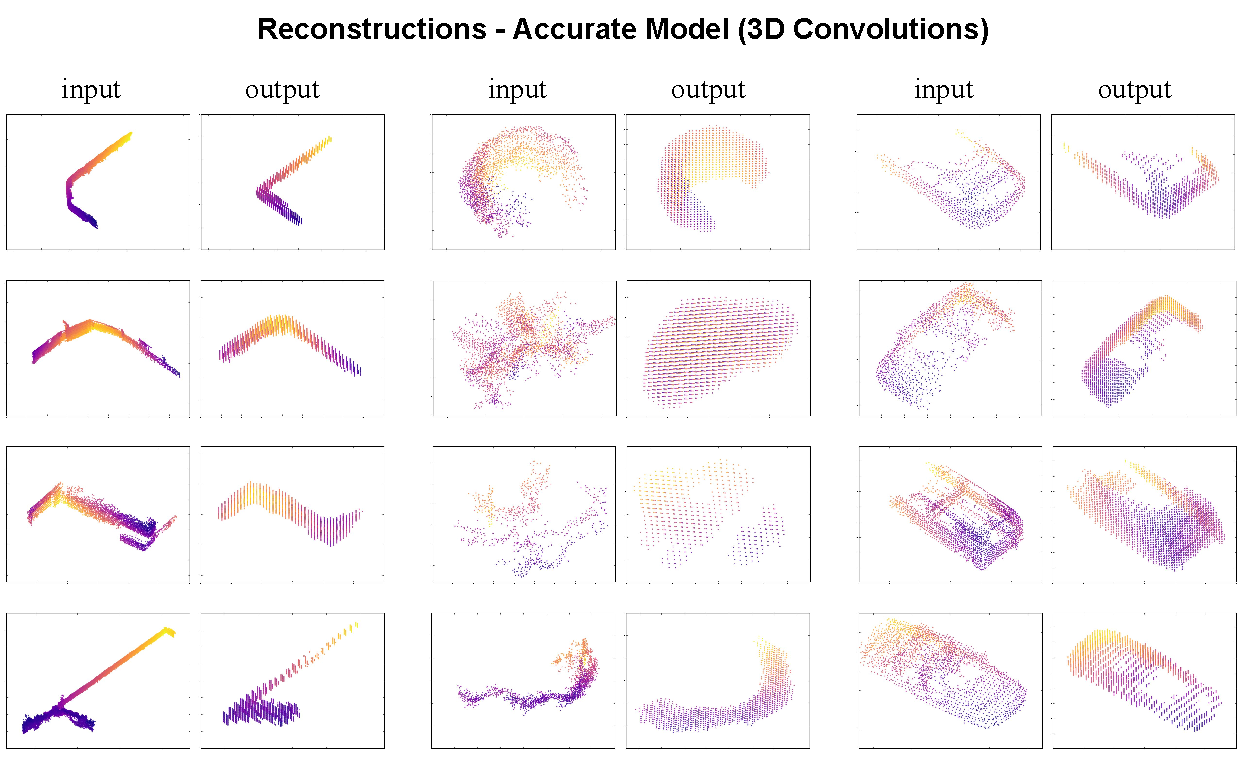
\includegraphics[width=5.2in]{images/convreconstructions.pdf}
  \caption{A few arbitrary selected reconstruction examples, for segments extracted from the KITTI database. The reconstructions in this figure were generated by the accurate model.}
  \label{fig:conv-reconstr}
  \hfill
  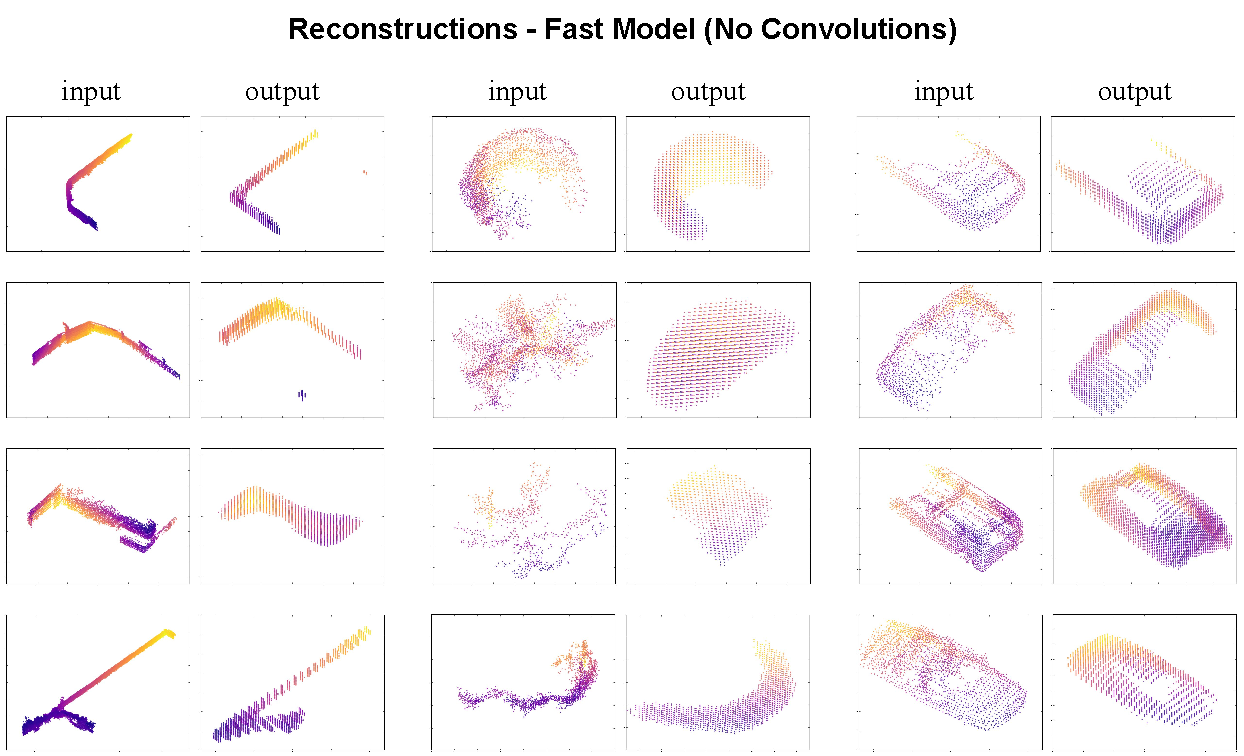
\includegraphics[width=5.2in]{images/noconvreconstructions.pdf}
  \caption{A few arbitrary selected reconstruction examples, for segments extracted from the KITTI database. The reconstructions in this figure were generated by the fast model. At first glance, the reconstructions are similar to the convolutional model reconstructions (Fig.\ref{fig:conv-reconstr}), which indicates that the fast model is adequate despite its simpler architecture. Looking at details however, inferior reconstruction quality is visible for most examples.}
  \label{fig:noconv-reconstr}
\end{figure}

A preprint paper by Brock et al.  \cite{voxel-autoencoder}, published while this project was underway,  mentions successful results on datasets using Variational Autoencoders for reconstructing Voxelized 3D data.
Brock et al. \cite{voxel-autoencoder} report that ``The model attains a 99.39\% true positive and 92.36\% true negative reconstruction accuracy on the ModelNet10 test set, indicating that it learns to reconstruct with high fidelity, but tends to slightly overestimate the probability of a voxel being present. ''\\

In our own experiments, we run the autoencoder on an arbitrary voxelized segment, producing a voxelized reconstruction. The reconstruction is then passed as input to the autoencoder, outputting a reconstruction-reconstruction, and so on 60 times. The goal was to see if the reconstructions tended to converge to a particular shape. We observed that with every iteration, the output prediction contains on average more occupied voxels, resulting in a final reconstruction which is a completely filled voxel. This agrees with the statement from Brock et al. \cite{voxel-autoencoder} quoted in the previous paragraph, which observes that the model ``tends to slightly overestimate the probability of a voxel being present.''\\

Experiments on the ModelNet database \cite{modelnet}, also show reconstruction results in accordance with Brock et al.'s observations.\\

It should be noted that an autoencoder model can be used not only encode and reconstruct (encode+decode) input data, as we do in this work, but also decode arbitrary description vectors. As such, it is possible to sample the latent space, and generate hallucinated segments. An example of such interpolation in the latent space is detailed in \citet{voxel-autoencoder}.

\subsection{Latent Space}
\label{subsec:latent_space}

In order to visualize the autoencoder latent space, t-Distributed Stochastic Neighbor Embedding (t-SNE) \cite{tsne} was used to project from n-dimensional to 2-dimensional space. \\

First, SegMatch was run on the KITTI drive 18 dataset, and the collected segments were extracted to a database. In addition, the matches found by SegMatch during this run were manually verified to be true matches between segments representing identical objects in the environment, and extracted. Labels were assigned by hand to segments, categorizing them into 4 classes, 'cars', 'walls', 'post', and 'unknown'. The 'unknown' class qualifies objects which were not recognized by a human. The results of t-SNE analysis on the segments' autoencoder encodings (fast architecture) are shown in Fig.~\ref{fig:tsne}. It should be noted that the scale features mentioned in Section \ref{sec:ae-implementation} are not included. In addition, the collected ground truth matches between segments were overlaid onto the t-SNE projection of their descriptions, as thin black lines collecting descriptions of matching segment pairs. The result is visible in Fig.~\ref{fig:tsne_matches}.\\

For comparison, the same process as in the above paragraph was applied to the same segments, using their eigenvalue-based descriptions instead of autoencoder descriptions. The resulting t-SNE projection and matches are visible in Fig.~\ref{fig:tsne_eig} and Fig.~\ref{fig:tsne_matches_eig} respectively.\\

In order to visualize the distribution of values in the autoencoder latent space, the encodings of a large number of segments were plotted, showing each segment's 15-value latent space representation as a stepfunction plot. This process was applied to both the fast architecture descriptions, and the accurate architecture descriptions. The resulting plots are displayed side-to-side in Fig.~\ref{fig:fastvaccurate_features}.\\

Another analysis of the latent space was made, looking at the average absolute value of each latent space dimension for segments with different labels. This was done in order to detect if particular classes were on average encoded closer to the origin in the 15-dimensional latent space. The resulting data is visible in Fig.~\ref{fig:avg_abs_features}.\\

\begin{figure}
  \centering
  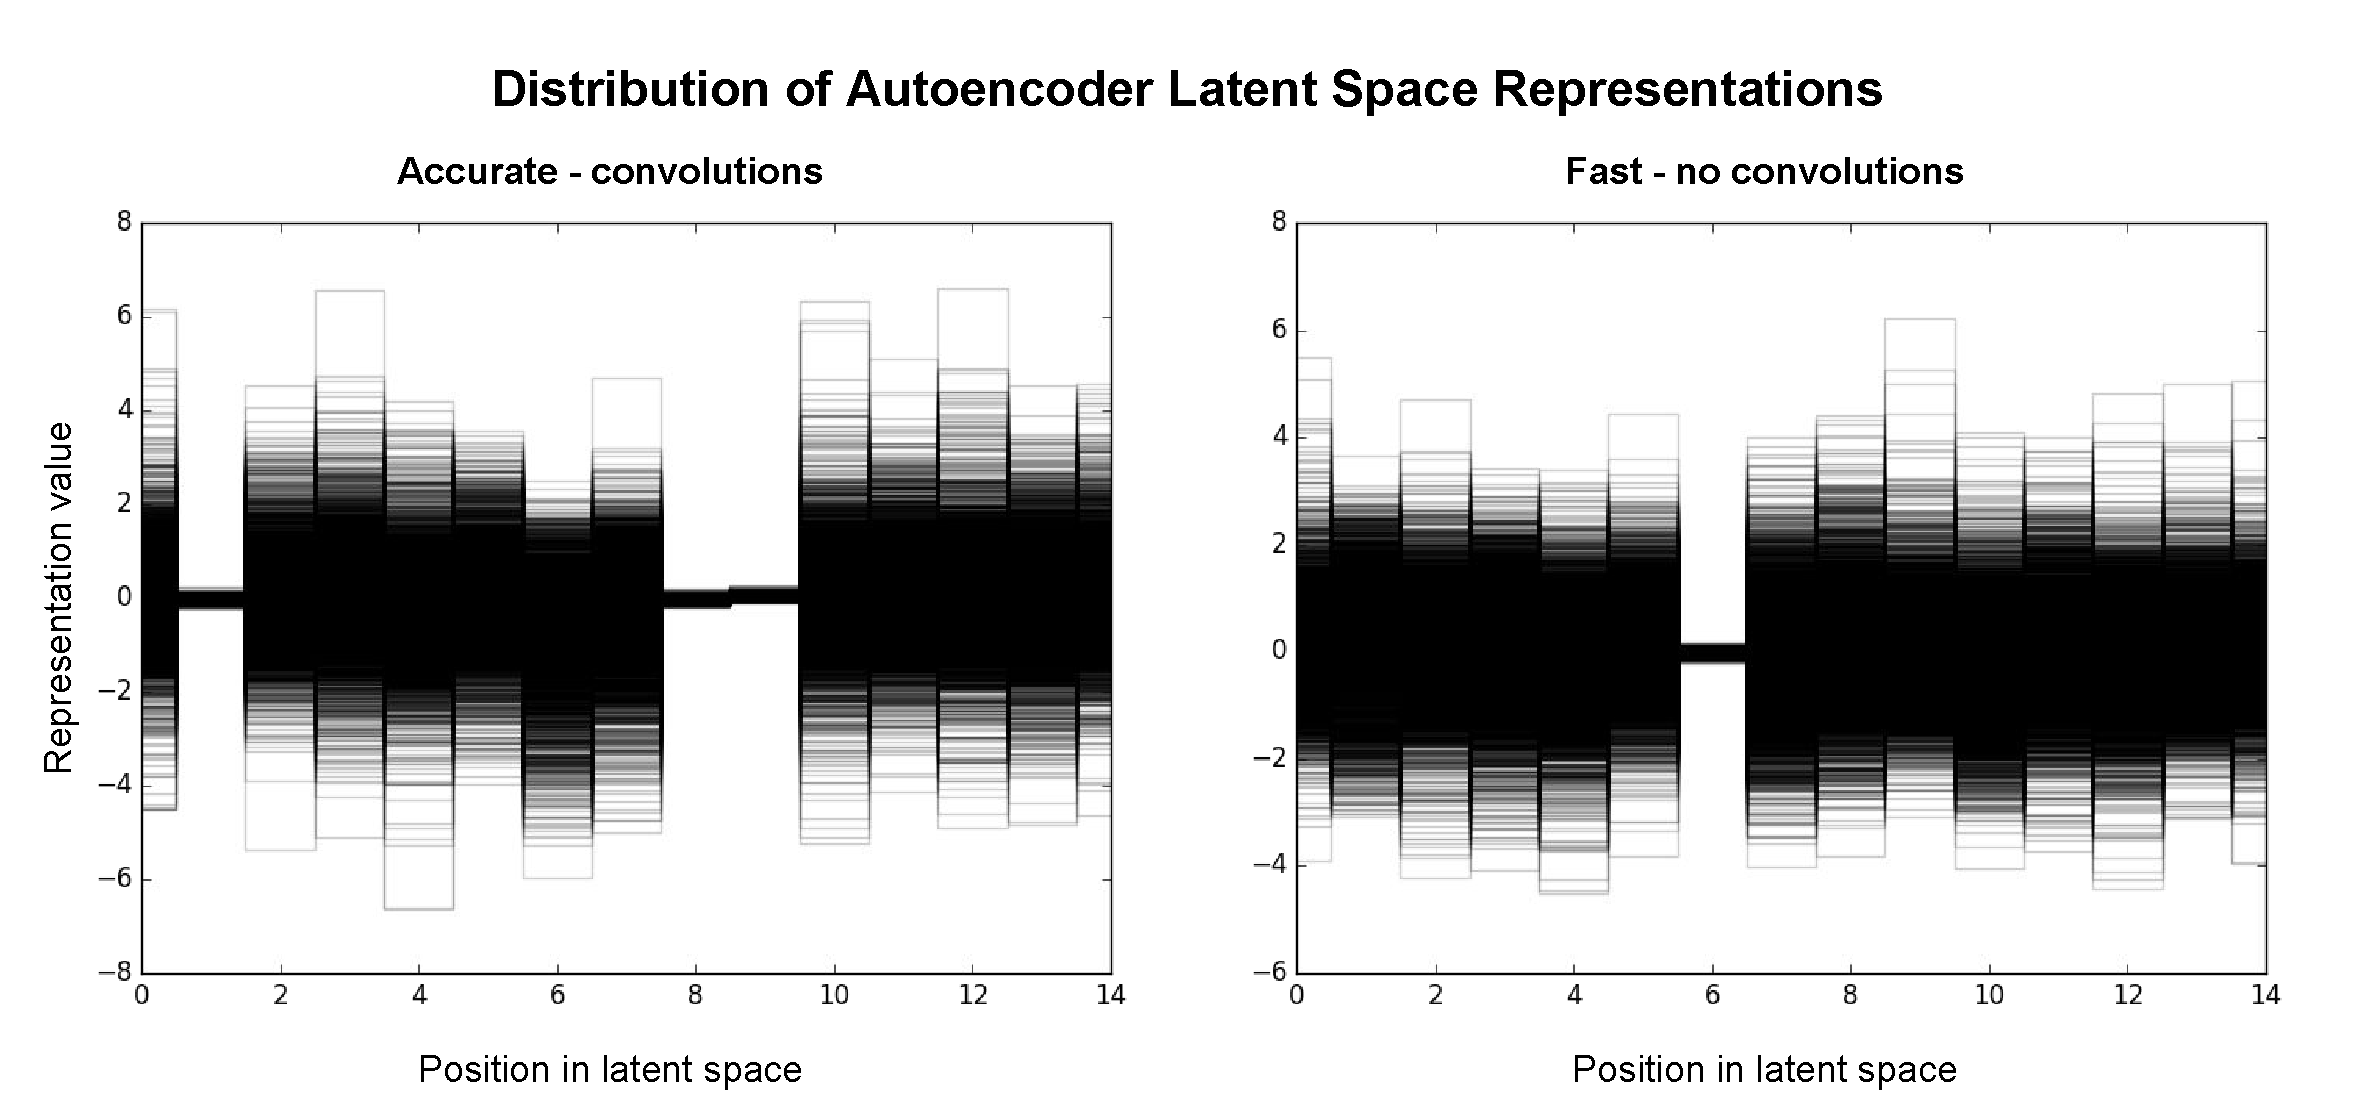
\includegraphics[width=5.2in]{images/fastvaccuratefeatures.pdf}
  \caption{Comparison of the latent space representations for 1187 segments extracted from the KITTI drive 18 dataset.}
  \label{fig:fastvaccurate_features}
\end{figure}

\begin{figure}
  \centering
  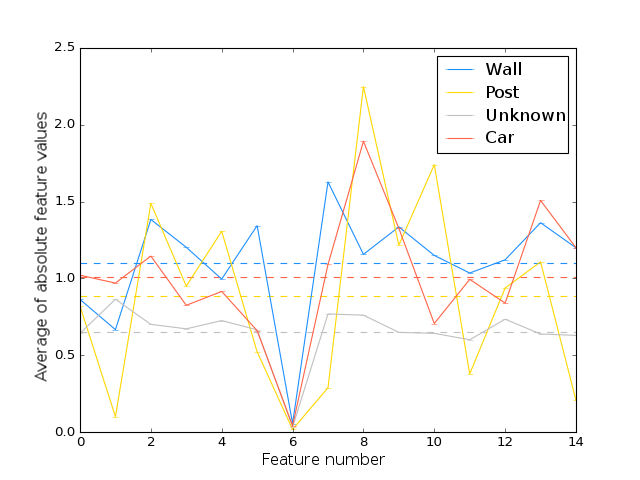
\includegraphics[width=5.2in]{images/avg_abs_features.png}
  \caption{Average absolute values of latent space representations for segments extracted from KITTI drive 18. Dashed lines reference the average of average absolute values across all features.}
  \label{fig:avg_abs_features}
\end{figure}

\begin{figure}[p]
  \centering
  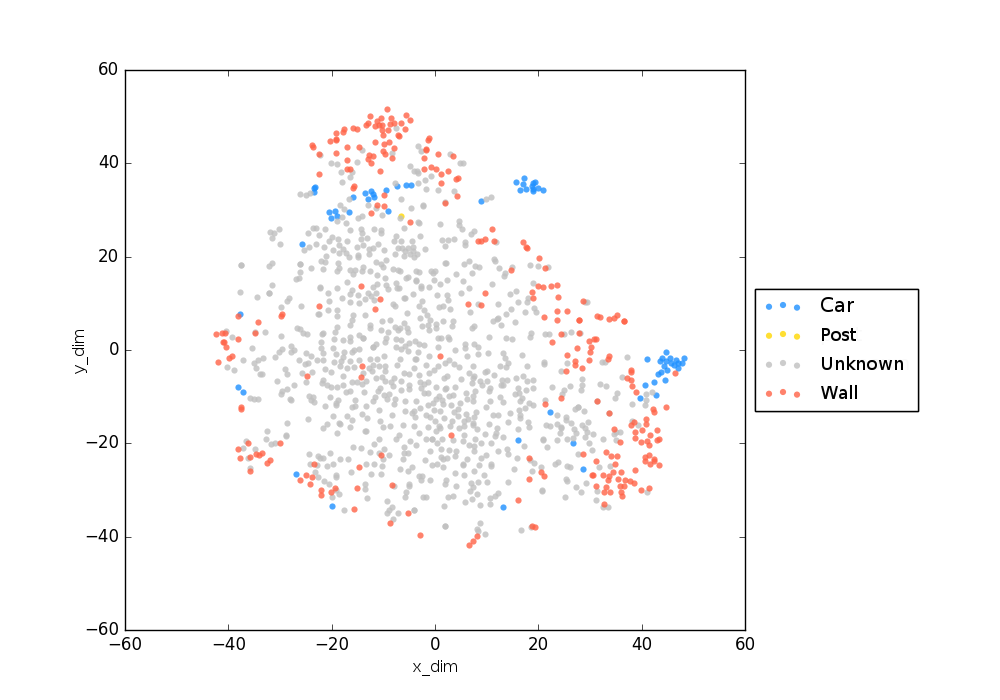
\includegraphics[width=5.2in]{images/t-sne.png}
  \caption{T-SNE projection of the latent space representations for 1187 segments extracted from the KITTI drive 18 dataset. The representations were generated using the fast autoencoder model.}
  \label{fig:tsne}
  \hfill
  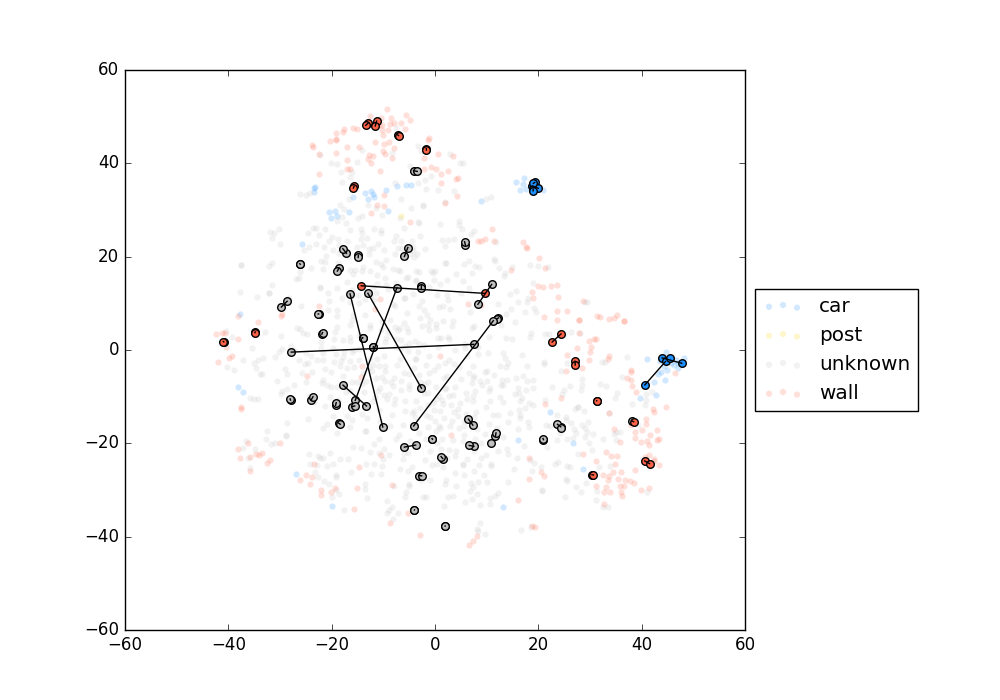
\includegraphics[width=5.2in]{images/t-sne_matches.png}
  \caption{Segment ground truth matches collected during the KITTI drive 18 run, overlaid on the t-SNE projection of their autoencoder description.}
  \label{fig:tsne_matches}
\end{figure}

\begin{figure}[p]
  \centering
  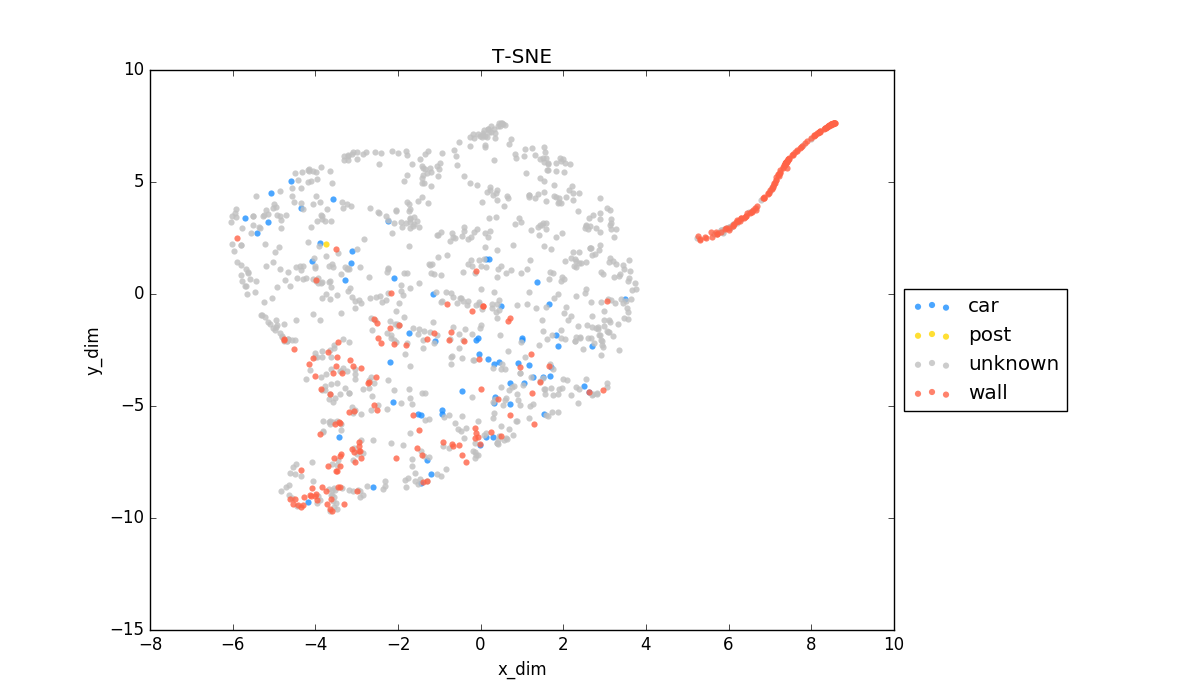
\includegraphics[width=5.2in]{images/t-sne_eig.png}
\caption{T-SNE projection of the eigenvalue descriptions for the same 1187 segments as in Fig.~\ref{fig:tsne}}
  \label{fig:tsne_eig}
  \hfill
  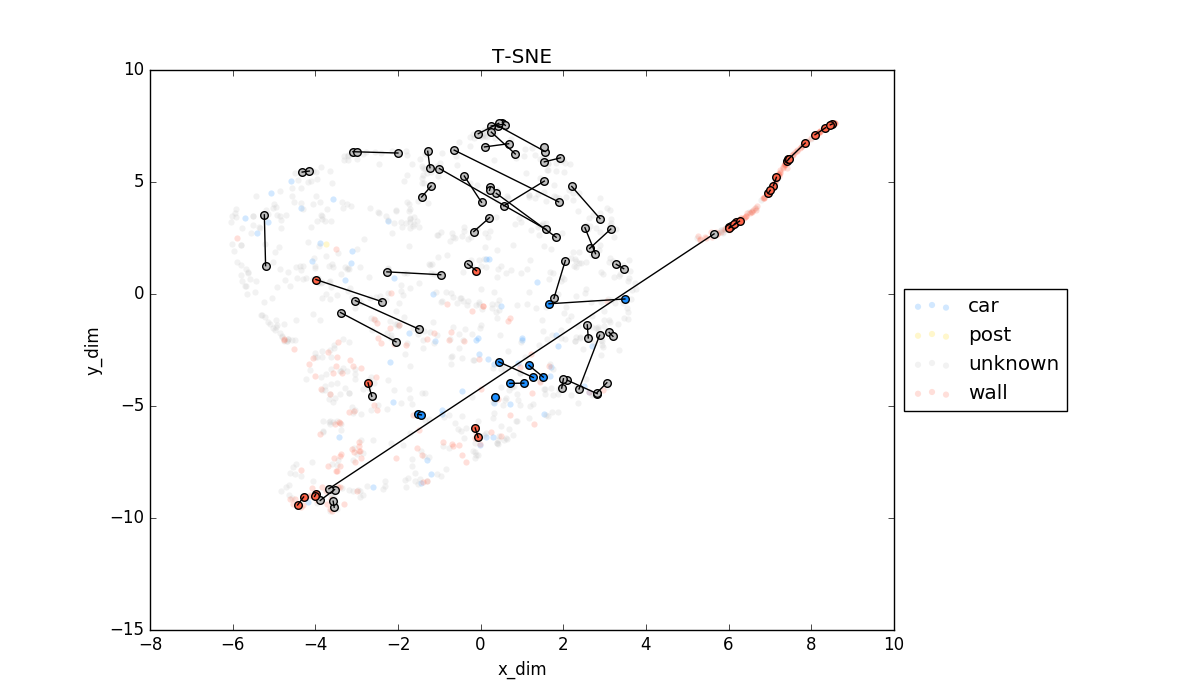
\includegraphics[width=5.2in]{images/t-sne_matches_eig.png}
\caption{Segment ground truth matches collected during the KITTI drive 18 run, overlaid on the t-SNE projection of their eigenvalue-based description.}
  \label{fig:tsne_matches_eig}
\end{figure}


An intuition is that the accurate architecture, due to having 3D convolutions, would be able to more efficiently compress segment representations in the latent space. Our observations show that on average the accurate model keeps 3 latent dimensions unused, whereas the fast model keeps 1 dimension unused (see Fig.~\ref{fig:fastvaccurate_features}). This goes in accordance with our expectations.\\

The KL-Divergence term in the variational Bayes autoencoder loss function acts as a regularizer, penalizing high values of the latent space predictions unless they lead to improved reconstruction cost. As a simplification, this means that the latent space values tend to be biased towards zero, while the reconstruction error makes them biased towards clusters of similar segments.\\

The latent space bias towards zero is responsible for the unused features seen in Fig.~\ref{fig:fastvaccurate_features}. Another consequence of this bias, is the fact that segments which the autoencoder can not recognize and reconstruct with high confidence tend to show lower average values overall in the latent space (visible in Fig.~\ref{fig:avg_abs_features}: segments of unknown class are harder to recognize for both human and autoencoder, as many resemble random 3d noise.)


\subsection{In-the-loop Results}

An experiment was run in order to compare the SegMatchAE algorithms versus the standard SegMatch algorithm (eigenvalue-based description). In this experiment, all parameters were kept identical for both trials, which were performed on the same dataset. The only difference between trials being the description and matching algorithms used (eigenvalues + knn + RF vs. autoencoder + knn). In order to capture statistically significant measures of performance, 100 trials were performed for each algorithm. These were performed in real-time to ensure practical usefulness. The observed performance measure was the amount of successful loop closures found by each algorithm.\\ 

A notable parameter value for this experiment was a relatively low nearest neighbour tolerance ($k=2$). This value was selected in order to limit the influence of geometric consistency filtering on the results. For other parameters (segmentation radius, spatial frequency, etc.), usual values (which were empirically set to obtain good performance) were selected.\\

The experiment results are shown in Fig.~\ref{fig:kitti20_performance}. The total amount of true-positive loop closures detected using the autoencoder description module is 1.6 times the amount detected using the eigenvalue description. In addition, the following ratios of false to true loop closures were measured:\\

Autoencoder + knn false-to-true loop-closure ratio: 0.0228\\
Eigenvalues + knn + RF false-to-true loop-closure ratio: 0.0223\\

\begin{figure}
  \centering
  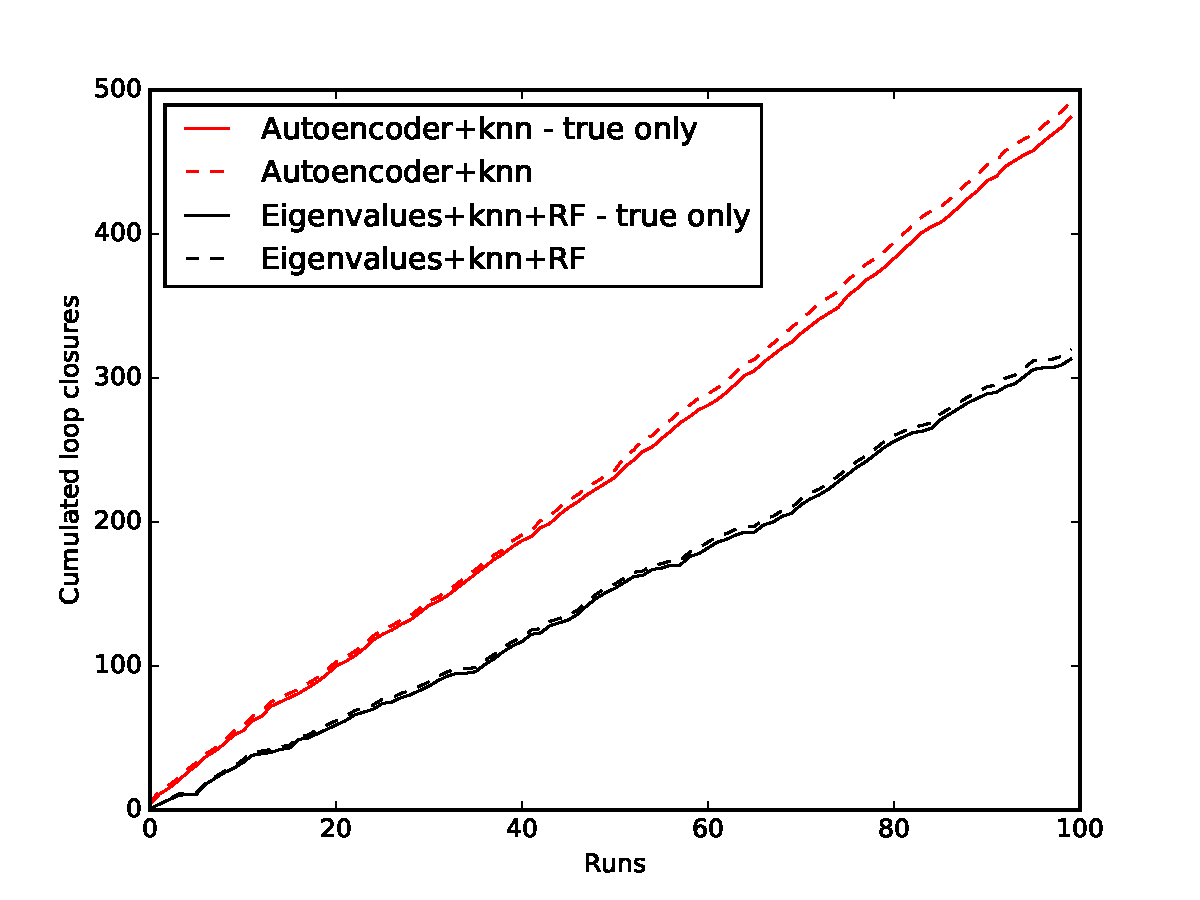
\includegraphics[width=5.2in]{images/kitti20performance.pdf}
  \caption{Comparison of the accumulated number for detected loop closures during 100 runs of SegMatch on the same dataset (KITTI drive 20). The trend shows that the loop-closure detection rate using the autoencoder module is 1.6 times higher than with the eigenvalue-based baseline. The ratio of false-to-true loop closure is measured to be identical (within 0.05\%) for both methods.}
  \label{fig:kitti20_performance}
\end{figure}

We believe that this experiment favors the hypothesis that the autoencoder models trained in this project indeed produce useful and distinct segment descriptions. Fig.\ref{fig:kitti20_performance} illustrates that the autoencoder as a descriptor for matching segments and closing loops outperforms the eigenvalue based descriptor.\\
